\documentclass[a3paper]{article}
\usepackage{graphicx}

% Fonts
\usepackage{fontspec}
\usepackage{unicode-math}
\setmainfont[Ligatures=TeX]{Libertinus Serif}
% \setmathfont[Ligatures=TeX]{Libertinus Math}
\setsansfont[Ligatures=TeX]{Libertinus Sans}
\setmonofont[Ligatures=TeX,Scale=0.95]{Libertinus Mono}

% color
\usepackage{xcolor}

% Links
\usepackage{hyperref}
\hypersetup
{
    linktoc=all,
    colorlinks,
    linkcolor={red!50!black},
    citecolor={blue!50!black},
    urlcolor={blue!80!black}
}

% Custom Lists
\usepackage{enumitem}

\usepackage{listings, listings-rust}
\definecolor{backcolor}{rgb}{0.95,0.95,0.95}

\usepackage{forest}

% Bibliography
\usepackage[
backend=biber,
style=ieee,
sorting=ynt
]{biblatex}
\bibliography{/home/chris/Documents/Bibliography/references}

% Math
\usepackage{amsmath}
\newcommand*\BitAnd{\mathbin{\&}}
\newcommand*\BitOr{\mathbin{|}}
\newcommand*\ShiftLeft{\ll}
\newcommand*\ShiftRight{\gg}
\newcommand*\BitNeg{\ensuremath{\mathord{\sim}}}

\usepackage{subfiles} % Best loaded last in the preamble

\newcommand{\figref}[1]{(βλ. \hyperref[#1]{Σχήμα~\ref{#1}})}

\begin{document}

\subfile{frontpage}
\newpage
\subfile{toc}
\newpage
\subfile{abstract}
\newpage

\section{Εισαγωγή}

Τα συστήματα αυτοματισμού είναι πλέον μέρος της καθημερινότητας
μας. Συναντάμε συνέχεια, χωρίς απαραίτητα να το συνειδητοποιούμε
κάποιου είδος σύστημα το οποίο είναι προγραμματισμένο να εκτελεί μια
διεργασία με βάση ορισμένες συνθήκες του εξωτερικού του
περιβάλλοντος. Το παραπάνω έχει μεγάλο αντίκτυπο στον κόσμο το οποίο
γίνεται ξεκάθαρο με την ραγδαία εξέλιξη του IoT (Internet of Things).
Περιτριγυριζόμαστε από συσκευές οι οποίες λειτουργούν ως συστήματα
αυτοματισμού αλλά παράλληλα επικοινωνούν με το Cloud.

Λόγο των περιορισμένων πόρων των συσκευών IoT έχουμε υιοθετήσει
συγκεκριμένα standards για τις γλώσσες προγραμματισμού και κατά
συνέπεια τα οικοσυστήματα που χρησιμοποιούμε για την κατασκευή
τους. Συνήθως αυτά τα standards είναι ένας συμβιβασμός μεταξύ ευκολίας
προγραμματισμού και πλήρης βελτιστοποίησης των πόρων της συσκευής. Με
ευκολία προγραμματισμού εννοούμε για παράδειγμα την αυτόματη
διαχείριση μνήμης (Garbage Collection). Δεν είναι σπάνιο πλέον να
βρίσκεται κάπου ένας μικροελεγκτής ο οποίος είναι ικανός να τρέξει ένα
runtime της Python ή της Java διευκολύνοντας κατά μεγάλο βαθμό την
διαδικασία υλοποίησης και της ασφάλειας όσο αναφορά την μνήμη. Έχουν
όμως προφανώς συνέπειες στην απόδοση του προγράμματος, τόσο μεγάλες
που ανάλογα με τις ανάγκες του έργου ενδέχεται να μην είναι
ρεαλιστικές επιλογές. Μάλιστα οι επιλογές τέτοιου τύπου γλωσσών έχουν
συχνά άλλα προβλήματα. Σε μεγάλα projects δεν είναι τόσο καλή πρακτική
η χρήση dynamic typing της Python καθώς ανοίγουν την πόρτα για πολλά
logic bombs ή άλλα λογικά σφάλματα. Από την άλλη στην Java, αν και
παρέχει στατικά types ο τρόπος διαχείρισης σφαλμάτων είναι, στην
καλύτερη περίπτωση, περιοριστικός. Για αυτούς τους λόγους αρχικά
φαίνεται ότι η C και η C++ κυριαρχούν στην πλειοψηφία των καταστάσεων
σε αυτόν τον τομέα, δίνοντας πλήρης έλεγχο στον προγραμματιστή
επιτρέποντας του να γράψει τον καλύτερο δυνατό κώδικα. Με την σειρά
του αυτό ανοίγει άλλες πόρτες σφαλμάτων και πιθανών κινδύνων ασφάλειας.
Σε μια πασίγνωστη παρουσίαση της Microsoft υποστηρίζετε ότι το 70\%
των ευαλωτήτων ασφάλειας τους οφείλονται σε προβλήματα διαχείρισης
μνήμης \cite{catalin_microsoft_nodate} \cite{thomas_proactive_nodate}
ενώ η σχετικά πρόσφατη δημοσίευση της αμερικάνικης κυβέρνησης προωθεί
την χρήση των ασφαλών γλωσσών προγραμματισμού
\cite{ann_marie_corvin_world_nodate} για αυτόν ακριβώς τον λόγο. Η
Rust, με το μοντέλο Aliasing XOR Mutability, είναι μια ξεκάθαρη λύση και αν
και δεν είναι σε καμία περίπτωση τέλεια αναφέρετε πολύ συχνά ως μια
μοντέρνα εναλλακτική της C/C++. 

Ο σκοπός της εκάστοτε εργασίας είναι να εξετάσουμε το παραπάνω ζήτημα,
να κατανοήσουμε και να συγκρίνουμε τρία διαφορετικά οικοσυστήματα
(Arduino,ESP-IDF,Embassy) ένα από τα οποία βασίζετε στην Rust
(Embassy). Θα χρησιμοποιήσουμε τον μικροελεγκτή ESP32C6-DEVKITC-1, τον
οποίο από εδώ και πέρα θα αναφέρουμε ως ESP και θα συγκρίνουμε τα
αποτελέσματα με βάση την υπολογιστική ισχύς (CPU Usage), αποθηκευτικό
χώρο και μνήμη κατά την εκτέλεση που χρησιμοποιεί το κάθε ένα. Παράλληλα
θα εξεταστεί το λεγόμενο "ease of development" αλλά όχι άμεσα,
προτιμώντας να περιγράψουμε πλήρως την λειτουργικότητα κάθε οικοσυστήματος χωρίς
προσωπικές απόψεις καθώς είναι η διευκόλυνση είναι προφανώς υποκειμενική.

Με σκοπό την πλήρης διαφάνεια των αποτελεσμάτων και γενικά της πληροφορίας
που βρίσκεται στο παρών κείμενο αξίζει να σημειωθεί ότι αναφέρονται πολλές
πτυχές της πληροφορικής εδώ. Από την πρακτική αρχιτεκτονική υπολογιστών μέχρι
και την θεωρητική μηχανή Turing αναφέρονται όλα με την πρόθεση ότι ο αναγνώστης
είναι υπεύθυνος να εκλάβει την χρησιμότητα, ανάγκη ή εγκυρότητα των παρακάτω αναφορών
όπως εκείνος πιστεύει. Είναι εκτός από τα πλαίσια αυτής της εργασίας η πλήρης περιγραφή
ορισμένων κλάδων και κατά συνέπεια πολλές λεπτομέρειες αφαιρόυντε, προφανώς όμως παρέχετε
η κατάλληλη βιβλιογραφία η οποία αναπαριστά αυτήν την γνώση πολύ καλύτερα από ότι θα μπορούσε
το παρών γραπτό.

\subsection{Συστήματα Αυτοματισμού}

\begin{figure}[h!]
\centering
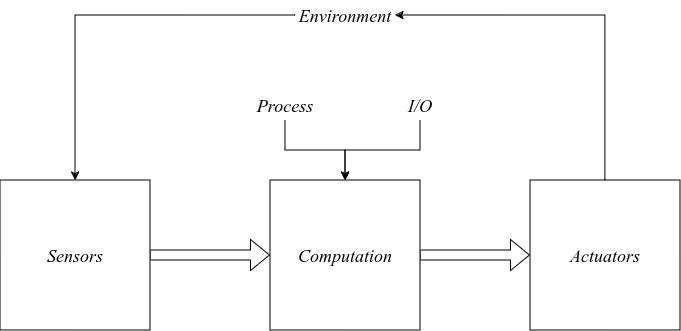
\includegraphics[scale=0.4]{images/introduction/as_elements.png}
\caption{Αναπαράσταση βασικών στοιχείων συστημάτων αυτοματισμού.}
 \label{fig:as_elements}
\end{figure}

Ένα σύστημα αυτοματισμού είναι ένα σύστημα που αποτελείτε από τρία
βασικά στοιχεία:

\begin{enumerate}
\item Τους σένσορες ή αισθητήρες, που λαμβάνουν δεδομένα από το
εξωτερικό τους περιβάλλων και παράγουν ένα όσο το δυνατόν πιο
αξιόπιστο αναλογικό ή ψηφιακό σήμα.
\item Ένα υπολογιστικό σύστημα, για παράδειγμα έναν μικροελεγκτή το
οποίο μπορεί να χρησιμοποιήσει το σήμα των αισθητήρων για
υπολογισμούς, επεξεργασία ή I/O.
\item Το στοιχείο δράσης ή ενεργοποιητής, που με βάση των υπολογισμών
του υπολογιστικού συστήματος ενεργοποιούνται ή παραμένουν
αδρανής. Αυτό το στοιχείο αποτελεί την έξοδο του συστήματος
αυτοματισμού και είναι αυτό το οποίο έχει συνήθως αντίκτυπο στο
εξωτερικό του περιβάλλων.
\end{enumerate}

Το υπολογιστικό σύστημα μπορεί να χρησιμοποιηθεί για να παίρνει
αποφάσεις με βάση των τιμών που δέχεται από τους αισθητήρες και εκεί
φαίνεται η πραγματική χρησιμότητα των αυτόματων συστημάτων. Πολλές
φορές με βάση την λήψη αποφάσεων (υπολογισμών) το αποτέλεσμα του
στοιχείου δράσης χρειάζεται να επιστρέψει στην είσοδο του συστήματος,
για παράδειγμα εάν χρειάζεται να ρυθμιστεί ένας σένσορας δυναμικά. Σε
αυτήν την περίπτωση το σύστημα λέγεται σύστημα ανατροφοδότησης ή
αλλιώς σύστημα κλειστού βρόχου \figref{fig:as_feedback}.

\begin{figure}[h!]
\centering
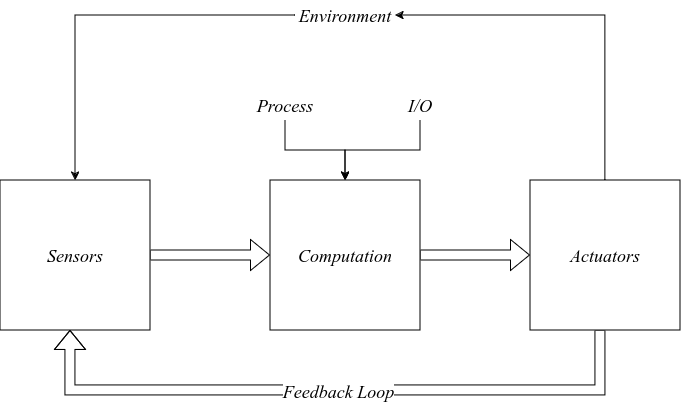
\includegraphics[scale=0.4]{images/introduction/as_feedback.png}
\caption{Σύστημα κλειστού βρόχου.}
 \label{fig:as_feedback}
\end{figure}

Το υπολογιστικό σύστημα στην δικιά μας περίπτωση είναι ο ESP. Έστω ότι έχουμε και έναν
αισθητήρα απόστασης HC-SR04. Μπορούμε να θεωρήσουμε ότι ο ενεργοποιητής
είναι η ενσωματωμένη κεραία του WiFi που κάθε λίγο χρονικό διάστημα επικοινωνεί ασύρματα
με ένα Router για να στείλει δεδομένα στο Cloud. 

\begin{figure}[h!]
\centering
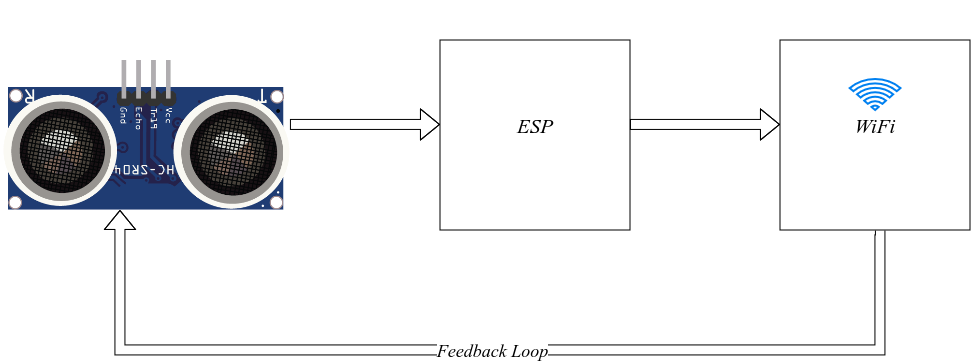
\includegraphics[scale=0.4]{images/introduction/thesis_as.png}
\caption{Αυτόματο σύστημα παρούσας περίπτωσης.}
 \label{fig:thesis_as}
\end{figure}

Οι σένσορες είναι τις περισσότερες φορές απλά ολοκληρωμένα κυκλώματα
(integrated circuits) τα οποία κάνουν κάποιου είδους μετρήσεις στο
εξωτερικό περιβάλλων. Ο αισθητήρας απόστασης αποτελεί καλό παράδειγμα
καθώς η λειτουργία του είναι εύκολα κατανοητή. Μόλις το trigger pin
λάβει σήμα HIGH ($5V$) για τουλάχιστον $10us$ ο σένσορας ενεργοποιείται
στέλνοντας 8 κύματα υπερήχου συχνότητας $40kHz$. Η αντανάκλαση του
ήχου έχει ως αποτέλεσμα το echo pin να μεταβεί με την σειρά του σε
κατάσταση HIGH. Εφόσον η ταχύτητα του ήχου είναι σταθερή και έχουμε την ικανότητα
να μετρήσουμε τον χρόνο για τον οποίο το echo pin διατηρείτε σε κατάσταση υψηλής
τάσης μπορούμε να μετρήσουμε την απόσταση μέσο $\text{velocity}= \frac{Δx}{Δt}$.
Για να τον συνδέσουμε στην ίδια διάταξη κυκλώματος με τον μικροελεγκτή πρέπει
να συνδέσουμε τα pins VCC,Trig,Echo,Gnd στα αντίστοιχα GPIO pins όπως φαίνεται
παρακάτω \figref{fig:schematic}.

\begin{figure}[h!]
\centering
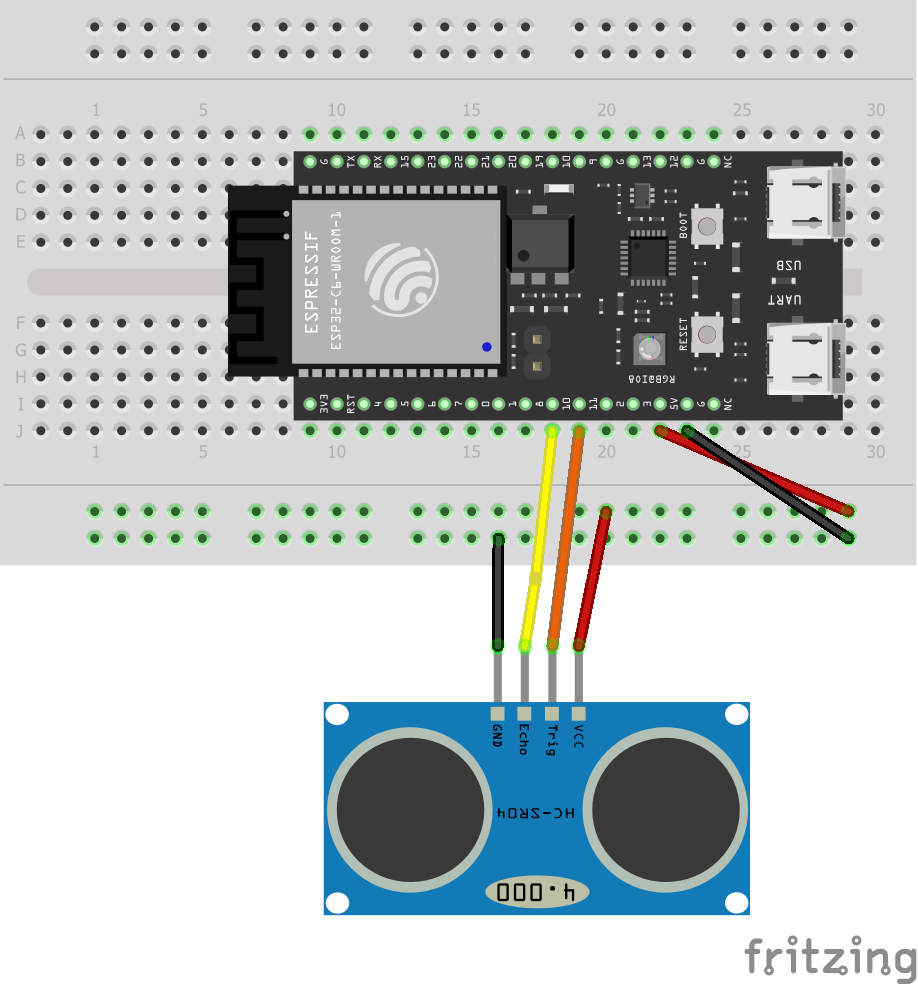
\includegraphics[scale=0.3]{images/introduction/thesis_schematic.png}
\caption{Παρούσα διάταξη.}
 \label{fig:schematic}
\end{figure}

\subsection{Embedded Systems}

Ο πιο σύγχρονος τρόπος προγραμματισμού παίρνει μέρος συνήθως σε αυτό
που αποκαλούμε user-space ενός λειτουργικού συστήματος.  Στο
user-space το OS (Operating System) αναλαμβάνει ένα πολύ μεγάλο μέρος
της πολυπλοκότητας του προγραμματισμού. Η δημιουργία εικονικής μνήμης,
η δυνατότητα παράλληλου προγραμματισμού, η διαχείριση μνήμη σορού
(heap memory) είναι όλα προβλήματα που αντιμετωπίζονται σχεδόν
αυτόματα πλέον. Επίσης μέσο του λειτουργικού συστήματος αποκρύβονται
οι λεπτομέρειες του hardware, τα πάντα σχεδόν προσφέρονται ως ψηφιακά
API (Application Programming Interface), τα οποία χτίζονται το ένα
πάνω στο άλλο.  Με κάθε πρόσθεση επιπέδου αφαίρεσης χάνετε λίγο
παραπάνω η ικανότητα πλήρης διαχείρισης του hardware με το θετικό ότι
σε γενικές γραμμές κάνει την ζωή του προγραμματιστή πιο εύκολη. Είναι
ξεκάθαρο λοιπόν ότι τα abstraction layers είναι χρήσιμα, αλλά είναι
δίκοπο μαχαίρι. Από την μια πλευρά η υλοποίηση των περισσότερων
εφαρμογών γίνεται απίστευτα πιο εύκολη. Από την άλλη, τι γίνεται όταν
πραγματικά χρειαζόμαστε να επικοινωνήσουμε με το hardware που έχουμε
μπροστά μας;
Πολλές φορές υπάρχουν συστήματα που δεν μπορούν ή δεν χρειάζεται
να τρέξουν ένα ολόκληρο operating system. Πολλές φορές δεν έχουμε την
επιλογή να τρέξουμε κώδικα πάνω σε ένα abstraction. Για παράδειγμα,
συστήματα που βρίσκονται σε απλές συσκευές όπως θερμοστάτες και
ρολόγια όχι μόνο δεν είναι απαραίτητο να τρέχουν OS αλλά πολλές φορές
δεν είναι βέλτιστο. 
Αναφερόμαστε στα συστήματα που δεν χρησιμοποιούν παραδοσιακά OS  ως
embedded systems διότι τα βρίσκουμε συχνά ενσωματωμένα σε μεγαλύτερες συσκευές.

\subsubsection{Βασικές αρχές υπολογιστικών συστημάτων}

Συνήθως προγραμματίζουμε ένα embedded system στο κύριο μηχάνημα μας
(host machine) το οποίο είναι λογικά διαφορετικής αρχιτεκτονικής. Αυτό
σημαίνει ότι πρέπει να μετατρέψουμε τον πηγαίο κώδικα της high level
γλώσσας που χρησιμοποιούμε στην αντίστοιχη γλώσσα που καταλαβαίνει ο
εξωτερικός επεξεργαστής. Αυτή η διαδικασία λέγεται
cross-compiling. Μάλιστα είναι απαραίτητο να δώσουμε στο πρόγραμμα τις
απαραίτητες τοποθεσίες στην μνήμη στην οποία θα εκτελεί εντολές ή θα
αποθηκεύει στατικά δεδομένα, αυτή είναι δουλειά του
linker. Αναλυτικότερα ο πηγαίος κώδικας, μαζί
με ότι βιβλιοθήκες χρησιμοποιούνται περνάνε από τον compiler και
πρώτα προεπεξεργάζονται και ενώνονται σε μια δομή.
Μεταφράζονται αργότερα στην assembly που καταλαβαίνει το target
μηχάνημα και ο assembler τα μετασχηματίζει σε ένα ή περισσότερα
Relocatable Object αρχεία, δηλαδή συλλογές από bytes που
αντιπροσωπεύουν τον κώδικα στην target γλώσσα. Έπειτα τα object files
περνάνε από τον linker ο οποίος ανάλογα με τις ρυθμίσεις του οργανώνει
το αρχείο και προσθέτει απαραίτητα δεδομένα για να δημιουργήσει ένα
εκτελέσιμο για το target μηχάνημα πρόγραμμα, για παράδειγμα ένα ELF32 \figref{fig:compilation_stages}.

\begin{figure}[h!]
\centering
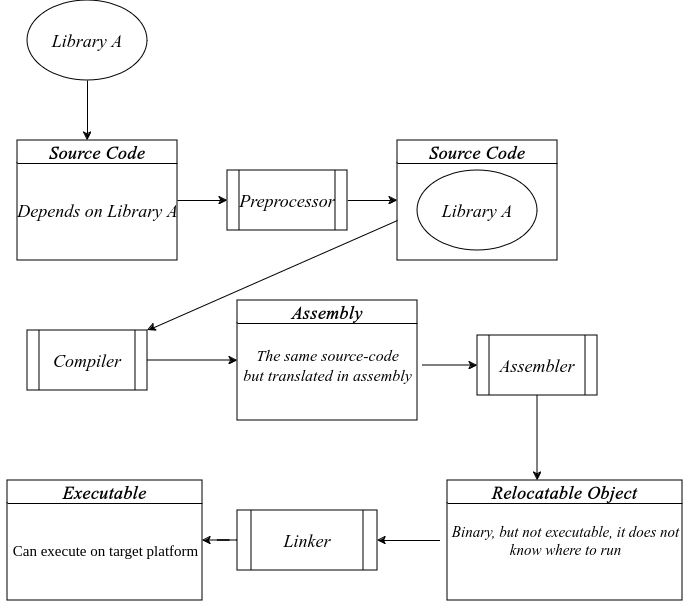
\includegraphics[scale=0.4]{images/introduction/compilation_stages.png}
\caption{Στάδια μεταγλώττισης.}
 \label{fig:compilation_stages}
\end{figure}

Η πραγματικότητα είναι ότι πλέον, ειδικά για μικρά projects, η διαδικασία
των σταδίων μεταγλώττισης είναι αυτοματοποιημένη και γίνονται όλα μέσο του
οικοσυστήματος όπως θα δούμε αργότερα. Όμως εξακολουθεί να είναι ιδιαίτερα χρήσιμη η γνώση
τους και απασχολεί πολύ τον κόσμο της πληροφορικής ακόμα και σήμερα, για λόγους βελτιστοποίησης 
και debugging.

Εφόσον έχουμε δημιουργήσει ένα εκτελέσιμο αρχείο πρέπει με κάποιο τρόπο να το στείλουμε στην συσκευή.
Συνήθως χρησιμοποιούμε κάποιο σειριακό πρωτόκολλο, τύπου USB το οποίο εσωτερικά συνδέεται με κάποιου είδους
μη πτητικής μνήμης για να το αποθηκεύσει \figref{fig:embedded_workflow}. Αυτό έχει ως αποτέλεσμα το πρόγραμμα να διατηρείτε ανεξαρτήτως
αν αργότερα κάνουμε επανεκκίνηση ή τερματίσουμε την συσκευή.

\begin{figure}[h!]
\centering
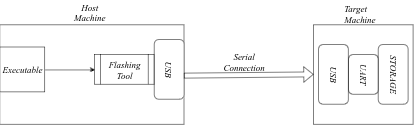
\includegraphics[scale=0.73]{images/introduction/programming_embedded.png}
\caption{Development workflow}
 \label{fig:embedded_workflow}
\end{figure}

Όταν ενεργοποιήσουμε την μηχανή τα απαραίτητα στοιχεία από την μη πτητική μνήμη
αντιγράφονται στην προσωρινή και ο καταχωρητής program counter του επεξεργαστή
δείχνει στην διεύθυνση μνήμης στην οποία βρίσκεται η πρώτη εντολή του πρώτου
προγράμματος που θα τρέξει. Συνήθως αυτό είναι κάποιου είδους bootloader, αλλά
στα ενσωματωμένα συστήματα δεν είναι πάντα αυτή η περίπτωση και τρέχει το firmware
που έχουμε γράψει κατευθείαν. 

\begin{figure}[h!]
\centering
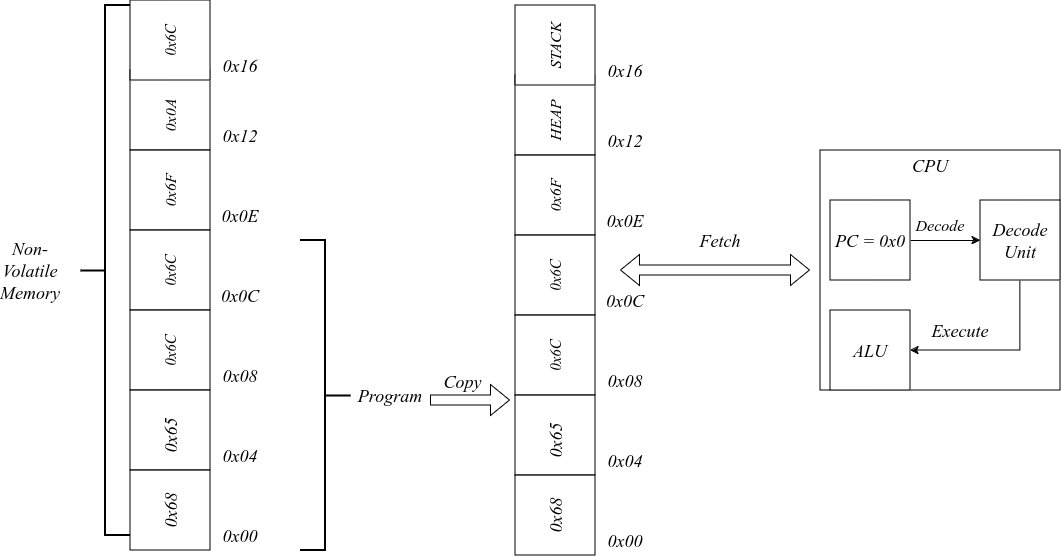
\includegraphics[scale=0.4]{images/introduction/instruction_cycle.drawio.png}
\caption{Κύκλος εντολών μηχανής}
 \label{fig:instruction_cycle_workflow}
\end{figure}

Αξίζει να σημειωθεί ότι δεν είναι πάντα ξεκάθαρο το πως η μη πτητική μνήμη αντιγράφετε στην
προσωρινή εξαρχώς, μπορεί οι μνήμες να έχουν ενσωματωμένο firmware και
να επικοινωνούν με σύνδεση τύπου I2C ή UART ή πιο λογικό να είναι ο
bootloader του επεξεργαστή σε μια ανεξάρτητη ROM (Read Only Memory)
σταθερής διεύθυνσης και μεγέθους και να είναι αυτός υπεύθυνος για την
επικοινωνία. Παράλληλα, υπάρχουν πολλοί καταχωρητές οι οποίοι διαχειρίζονται
την κατάσταση (state) του επεξεργαστή και κατά συνέπεια ολόκληρου του συστήματος. Ο program counter
αναφέρετε διότι διατηρείτε σε πρακτικά όλες τις αρχιτεκτονικές. 

Είναι σημαντικό να γνωρίζουμε επίσης ότι μια εντολή δεν εκτελείτε
κατευθείαν. Όπως αναπαριστά το παραπάνω διάγραμμα, πρώτα ο
επεξεργαστής διαβάζει την εντολή από την μνήμη (fetch). Έπειτα την
αποσπά για να την κατανοήσει (decode). Θυμόμαστε ότι έχουμε
αποθηκεύσει το εκτελέσιμο αρχείο, δηλαδή αυτό που είναι κατανοητό στην
μηχανή, σε δυαδική μορφή, όχι σε γραμματοσειρά που είναι κατανοητή
στους ανθρώπους. Για παράδειγμα οι εντολές της αρχιτεκτονικής RISC-V
32bit έχουν σταθερό μέγεθος και αναπαριστούν μια αριθμητική τιμή $x \in
[0, 2^{31}] \subseteq \mathbb{N}_0$. Ο αριθμός αυτός στην δυαδική του μορφή, μπορεί να
διαχωριστεί σε $n\in\mathbb{N}$ θραύσματα, συνήθως τα λέμε nibbles, μέσο bit operations και εξηγούν στον
επεξεργαστή τι πρέπει να κάνει. Στην πολύ συχνή εντολή
\verb|add t0, t1, t2|, στην οποία προσθέτουμε την τιμή του καταχωρητή
$t1$ με την τιμή του καταχωρητή $t2$ και την αποθηκεύουμε στον t0, ένα
unit του επεξεργαστή κάνει τις παρακάτω πράξεις για να την
αποκωδικοποιήσει.

\vspace{0.5cm}

\begin{math}
  Bits_{0-31} \text{ is stored in memory and then enters a unit capable of decoding RISC-V instructions:}  \newline
  Bits_{0-31} = \verb|add t0, t1, t2| = 0x007302b3_{(16)} \newline
  Bits_{0-6} = Bits_{0-31} \BitAnd 0x7F_{(16)} \rightarrow \text{opcode} \newline
  Bits_{7-11} = (Bits_{0-31} \ShiftRight 7_{(10)}) \BitAnd 0x1F_{(16)} \rightarrow \text{destination register} \newline
  Bits_{12-14} = (Bits_{0-31} \ShiftRight 12_{(10)}) \BitAnd 0x7_{(16)} \rightarrow \text{operation (addition)} \newline
  Bits_{15-19} = (Bits_{0-31} \ShiftRight 15_{(10)}) \BitAnd 0x1F_{(16)} \rightarrow \text{source register 1} \newline
  Bits_{20-24} = (Bits_{0-31} \ShiftRight 20_{(10)}) \BitAnd 0x1F_{(16)} \rightarrow \text{source register 2} \newline
  Bits_{25-31} = (Bits_{0-31} \ShiftRight 25_{(10)}) \BitAnd 0x7F_{(16)} \rightarrow \text{addition variant} \newline
\end{math}

Η λογική αποκωδικοποίησης είναι ίδια σε πρακτικά όλες τις
αρχιτεκτονικές όμως το μέγεθος μιας εντολής δεν είναι σε όλες
σταθερό. Τέλος, παίρνουν μέρος οι αριθμητικές πράξεις ή το I/O με βάση
τα αποτελέσματα του decoding (execute).

Η καθυστέρηση που έρχεται ως επίπτωση των παραπάνω πράξεων μπορεί να
φαίνεται στην αρχή σαν μεγάλη υπερφόρτωση του υπολογιστικού συστήματος
και πράγματι για παλαιότερες αρχιτεκτονικές ήταν. Το λεγόμενο
Instruction Cycle όμως (Fetch \rightarrow Decode \rightarrow Execute)
που μόλις αναλύσαμε έχει οριστεί για έναν πολύ συγκεκριμένο
λόγο. Πρόκειται για την τεχνική υλοποίησης "διοχέτευση" (pipelining).
Oυσιαστικά ο επεξεργαστής εκμεταλλεύεται την καθυστέρηση που παίρνει
μέρος υλοποιώντας μια δομή, για τους σκοπούς μας ένα pipeline που μπορεί να δεχθεί
μέχρι $ν \in \mathbb{N}$ εντολές. Κάθε
φορά που αλλάζει το state μιας εντολής προχωράει στο pipeline και
προσθέτετε μια καινούργια εντολή στην αρχικοποιημένη της
κατάσταση. Αυτό δίνει την ψευδαίσθηση παραλληλισμού στο επίπεδο εντολών του
επεξεργαστή και είναι ένας από τους πολλούς λόγους που σύγχρονα
προγράμματα μπορούν να τρέχουν τόσο γρήγορα χωρίς απαραίτητα να
τρέχουν πάνω σε ένα runtime.

\begin{figure}[h!]
\centering
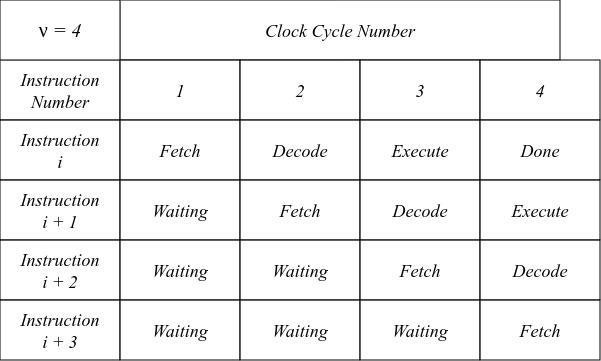
\includegraphics[scale=0.4]{images/introduction/pipelining.png}
\caption{Αναπαράσταση βασικών στοιχείων συστημάτων αυτοματισμού.}
 \label{fig:pipelining}
\end{figure}

Η περίπτωση του ESP32C6 είναι ότι αν και είναι πανίσχυρος για μικροελεγκτής ανάλογα
με το framework περιέχει μινιμαλιστικά, στην καλύτερη περίπτωση, abstractions.

\begin{figure}[!htb]
    \centering
    \begin{minipage}{0.49\textwidth}
        \centering
        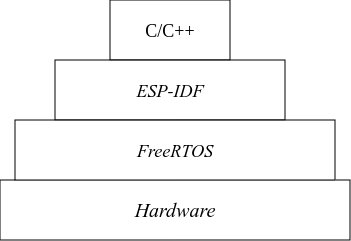
\includegraphics[scale=0.4]{images/introduction/idf_layers}
        \caption{ESP-IDF Abstraction Layers}
        \label{fig:idf_layers}
      \end{minipage}  
    \begin{minipage}{0.49\textwidth}
        \centering
        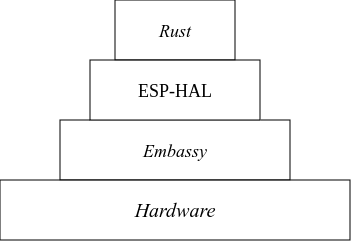
\includegraphics[scale=0.4]{images/introduction/rust_layers}
        \caption{Embassy Abstraction Layers}
        \label{fig:rust_layers}
      \end{minipage}  
    \begin{minipage}{0.49\textwidth}
      \centering
        \vspace{0.5cm}
        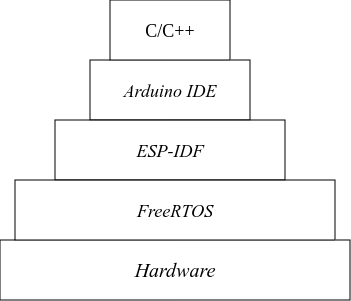
\includegraphics[scale=0.4]{images/introduction/arduino_layers}
        \caption{Arduino Abstraction Layers}
        \label{fig:arduino_layers}
    \end{minipage}%
\end{figure}

\subsubsection{ESP ως ενσωματομένο σύστημα}

\subsubsection{Μεταγλώττιση και Τύποι}


\section{Yλοποίηση Rust}


Για την υλοποίηση σε Rust είναι αρχικά σημαντικό να ξεκαθαρίσουμε ορισμένα
πράγματα. Ο μεταγλωττιστής της Rust παρέχει στην πραγματικότητα δύο ξεχωριστές
γλώσσες, την ασφαλής (safe) Rust και την μη ασφαλής (unsafe) Rust. Η safe Rust
όπως υπονοεί το όνομα είναι το μέρος της γλώσσας που χρησιμοποιεί στατική ανάλυση
για να αποτρέψει σύνηθες σφάλματα που αφορούν την διαχείριση μνήμης. Η unsafe Rust
ενεργοποιείται με την λέξη κλειδί \verb|unsafe| και επιτρέπει ενέργειες που ενδεχομένως
μπορούν να διακόψουν (halt) την εκτέλεση του προγράμματος, όπως να κάνουμε dereference έναν
σκέτο (raw) δείκτη. Η σύνηθες υλοποίηση της λογικής της Rust που εξηγείτε στα παρακάτω κεφάλαια
διατηρείτε και στις δύο εκδοχές της γλώσσας και όπως θα δούμε μπορούν προφανώς να συνυπάρχουν.

Σε γενικές γραμμές όμως η safe Rust είναι ένα υποσύνολο της unsafe Rust. Μάλιστα διαισθητικά
τουλάχιστον μπορούμε να πούμε πως η safe Rust είναι υποσύνολο της C. Δηλαδή έστω ότι όλα τα πιθανά
προγράμματα εκφράσιμα από μια παραδοσιασκή μηχανή Turing βρίσκονται στο σύνολο $U$, όλα τα πιθανά
προγράμματα εκφράσιμα από το specification της C $C=U$ και όλα τα πιθανά προγράμματα της safe Rust $SR \subseteq C$.
Συνεχίζοντας ισχύει ότι για την unsafe rust $UR=C=U, SR \subseteq UR$. 

Έχωντας πει αυτά γίνεται ξεκάθαρη η πολυπλοκότητα του μεταγλωτιστή. Σε σύγκριση με την C η οποία 
μπορεί να μεταφραστεί σε γλώσσα μηχανής με μόνο ένα ενδιάμεσο στάδιο η Rust χρειάζεται το λιγότερο 3
στην μόνη υλοποίηση που υπάρχει. Σε αυτά τα τέσσερα στάδια, δεν μετριούνται καν οι ενδιάμεσες αναπαραστάσης
του LLVM. Στο σχήμα \ref{fig:rust_ir} η κάθε ενδιάμεση αναπαράσταση μεταλλάζει τον πηγαίο κώδικα σε όλο και
μια πιο απλή γλώσσα που στο τέλος η μηχανή μπορεί να κατανοήσει.

\begin{enumerate}
\item HIR: Είναι ο πηγαίος κώδικας αλλά desugared, δηλαδή οντότητες όπως είναι ο χρόνος
  ζωής μεταβλητών (lifetimes) ή οι τύποι των μεταβλητών εκφράζονται πλέον ρητά. Ένα
  feature σημαντικού ενδιαφέροντος για εμάς που γίνεται desugared σε αυτό το στάδιο είναι τo
  \verb|async|.
\item THIR: Σε αυτήν την αναπαράσταση η απλοποίηση του κώδικα γίνεται πιο εμφανής. Σύνθετη
  τύποι μετατρέπονται σε πιο απλούς (primitives), τα generics μεταφράζονται στις στατικές τους
  μορφές και οι μέθοδοι μετατρέπονται σε συναρτήσεις.
\item MIR: Ο λόγος ύπαρξης του THIR είναι για να γίνεται πιο απλή η μετάφραση σε αυτό το στάδιο.
  Είναι ουσιασικά ένα Control-Flow Graph (CFG) που αναπαριστά την ροή εκτέλεσης του προγράμματος.
  Εδώ γίνεται η στατική ανάλυση απαραίτητη για τον Borrow Checker, τον εγκέφαλο του στατικού ελεγκτή
  της Rust που είναι υπεύθυνος για το specification που πρέπει να ακολουθεί το πρόγραμμα μας. 
\end{enumerate}

Η τελική μετατροπή είναι του LLVM το οποίο είναι ένα third-party framework που χρησιμοποιείτε ως
παγκόσμια γλώσσα μηχανής. Είναι μια υπερβολικά απλή και μινιμαλιστική γλώσσα προγραμματισμού βασισμένη
σε SSA (Static Single Assignment) η οποία μεταφράζεται στις πιο γνωστές αρχιτεκτονικές. Η SSA είναι ιδανική
για να αναπαραστήσει την Rust σε χαμηλότερο επίπεδο κυρίως για την ιδιότητα που έχει όσο αναφορά το code-locality.
Εδώ είναι καλή στιγμή να αναφερθούμε στο specification της Rust, τους κανόνες δηλαδή που ένα πρόγραμμα πρέπει να
ακολουθεί για να γίνει compile.


\begin{enumerate}
  \item Το πρώτο βασικό χαρακτηριστικό της γλώσσας είναι ότι τα σύμβολα είναι σταθερές by default, για να ορίσουμε μεταβλητές
    πρέπει να χρησιμοποιήσουμε την λέξη κλειδί \verb|mut|.    
\begin{lstlisting}[language=Rust]
let x = 5;
x = 6; //Error `x` is not mutable

let mut y = 5;
y = 6; // Valid, since its `mut`
    \end{lstlisting}
  \item Κάθε τιμή στη Rust έχει ένα και μόνο ένα owner. Όταν ο owner της τιμής βγαίνει εκτός
    scope η τιμή αποδεσμεύεται αυτόματα από τη μνήμη.    
\begin{lstlisting}[language=Rust]
fn main() {
    let s = String::from("hello"); 
    //Create inner scope
    {
    let t = s; //`t` now owns `s`
    }
  //Inner scope ends here
  println!("{}", s); // Error: `s` has been consumed/moved
}
\end{lstlisting}
\item Κάθε τιμή μπορεί να έχει άπειρες αμετάβλητες αναφορές $\&Τ$ ή μόνο μια μεταβλητή αναφορά
  $\&mut T$.  
\begin{lstlisting}[language=Rust]
let mut x = 10;
let y = &x; // Immutable reference 
let z = &x; // Valid, can have infinite 
println!("{},{}", y, z);

let w = &mut x; // Error: Cant `&mut T` while `&T` exist
\end{lstlisting}
\end{enumerate}

\begin{figure}[!htb]
    \centering
    
\includegraphics[scale=0.4]{images/rust/rust_irs.png}
    \caption{Rusts Intermediate Representations.}
    \label{fig:rust_ir}
\end{figure}

\newpage

\subsection{Λογική και Design Patterns}

\subsubsection{Γραμμική Λογική}

Η λογική είναι από τις σημαντικότερες αρχές της Rust καθώς
αποτυπώνει με αυστηρό μαθηματικό τρόπο τους υποκείμενους
μηχανισμούς του μεταγλωττιστή. Μάλιστα έχουμε ήδη αναφέρει ότι
όλες οι γλώσσες συμπίπτουν στη επιστήμη της λογικής με τον έναν
ή τον άλλον τρόπο, σε καμία περίπτωση όμως δεν είναι απαραίτητη
για την κατανόηση τους. Γιατί λοιπόν είναι εξαίρεση η Rust?
Η λέξη κλειδί είναι η αυστηρότητα της γλώσσας και η απαίτηση του
μεταγλωττιστή ένα πρόγραμμα να είναι σωστό με βάσει προορισμένους
κανόνες. Το σύστημα λογικής που χρησιμοποιείτε για να εκφράσει την
εγκυρότητα ενός προγράμματος είναι ένα υποσύνολο της γραμμικής λογικής
(Linear Logic).

Στις συνηθισμένες λογικές/γλώσσες προγραμματισμού χρησιμοποιούμε $\phi \vdash \psi$
εννοώντας ότι εφόσον ξέρουμε την εγκυρότητα του $\phi$ μπορούμε να συμπεράνουμε
την εγκυρότητα του $\psi$. Η σχέση αυτή διατηρείτε για πάντα, ανεξαρτήτως της
κατάστασης, μόλις αποδείξουμε ότι $\psi$ είναι αληθές επειδή το $\phi$ είναι
αληθές δεν μπορούμε ξαφνικά να αλλάξουμε γνώμη, $\phi \rightarrow true$ για
πάντα αλλιώς αλλάζει και το αποτέλεσμα του $\psi$. Αυτό έχει ως αποτέλεσμα
ορισμένα συμπεράσματα να είναι πολύ πιθανά, για παράδειγμα έστω $\Alpha \rightarrow \Beta,
\Alpha \rightarrow \Gamma$, τότε ένα ενδεχόμενο συμπέρασμα μπορεί να είναι $\Alpha \vdash \Beta \land \Gamma$.
Το παραπάνω παράδειγμα αν και συμβατό με την πραγματικότητα δεν μοντελοποιεί πλήρως
ένα \textbf{σωστό} πρόγραμμα. Αν το $\Alpha$ ήταν πρόσβαση σε έναν πόρο όπως ένα αρχείο
δεν μπορούμε να το επαναχρησιμοποιήσουμε και για το $\Beta$  και για το $\Gamma$, τι γίνεται
αν ένα από τα δύο απενεργοποιήσει τον πόρο ή στο παράδειγμα μας κλείσει το αρχείο? Χρειαζόμαστε
λοιπόν έναν τρόπο να ελέγχουμε για αυτές τις περιπτώσεις.

Η γραμμική λογική προσθέτει την έννοια της κατανάλωσης. Με $\Alpha \multimap \Beta$
εννοούμε ότι για \textbf{ένα} $\Alpha$ παράγετε \textbf{ένα} $\Beta$. Προσθέτοντας
επίσης έναν εναλλακτικό τελεστή για το "γραμμικό λογικό και" $\otimes$ ισχύει ότι:

\begin{center}
    \begin{math}
    \Alpha \multimap \Beta,\Alpha \multimap \Gamma, \Alpha \nvdash \Beta \otimes \Gamma
    \end{math}
\end{center}

Το $\Alpha$ καταναλώνετε από την πιο αριστερή οντότητα, κατά σύμβαση, το $\Beta$.
Με τον ίδιο συνειρμό ισχύει  $\Alpha \multimap \Beta,\Alpha \multimap \Gamma, \Alpha,\Alpha \vdash \Beta \otimes \Gamma$
καθώς τώρα έχουμε δύο οντότητες του $\Alpha$ η κάθε μια θα καταναλωθεί από το $\Beta$ και $\Gamma$ αντίστοιχα. Το γεγονός
ότι ο μεταγλωττιστής καταλαβαίνει την γραμμική λογική δεν σημαίνει ότι την αντικαθιστά οποιαδήποτε άλλη πλήρως.

Πολλές φορές είναι απαραίτητο να παραχθούν $v\in\mathbb{N} $ αναφορές (references) αμετάβλητης μορφής, δηλαδή ισχύει:

\begin{equation}
\alpha:T \rightarrow \beta: \&T
\end{equation}

Όμως δεν μπορούμε να έχουμε παραπάνω από μια αναφορά αν είναι μεταβλητή, σε αυτήν την περίπτωση καταναλώνετε:

\begin{equation}
\alpha:T \multimap \beta: \& mut T
\end{equation}

Το ίδιο ισχύει για οποιαδήποτε μη-αντιγράψιμη τιμή:

\begin{equation}
\alpha:T \multimap \beta: T
\end{equation}

Ορισμένοι τύποι όμως είναι υπερβολικά πολύ εύκολο να αντιγραφθούν χρησιμοποιόντας κάποιου είδους
\verb|memcpy|, για παράδειγμα \verb|u8|. Αυτοί οι τύπου είναι αντιγράψιμοι.

\begin{equation}
\alpha:T \textup{ is Copy } \rightarrow \beta:T
\end{equation}

Η έννοια της κατανάλωσης της γραμμικής λογικής είναι ίδια ακριβώς με την έννοια
της ιδιοκτησίας (ownership) της Rust. Παρακάτω είναι μερικά ακόμη παραδείγματα.

\begin{lstlisting}[language=Rust]
struct T;

fn reference_infinite_times(a: T) -> T {
    let b = &a;
    let c = &a;
    let d = &a;
    // let e = &mut a; Error, cant consume variable
    // that is referenced in its lifetime
    return a;
}

fn mutate_reference(mut a: &mut T) -> &mut T {
    let b = a;
    // return a; Error, use of consumed variable 'a'
    return b;
}

fn consume_and_return(a: T) -> T {
    let b = a;
    // let c = a; Error, use of consumed variable 'a'
    return b;
}

fn can_copy(mut a: u8) -> u8 {
    let b = a;
    let c = a;
    let d = &mut a;
    let e = &a;

    return a;
}

fn main() {
    let v0: T = T;

    let v1 = reference_infinite_times(v0);
    //infinite_references(var0); Error,
    //use of consumed variable 'v0'

    let mut v2 = consume_and_return(v1);
    //infinite_references(var1); Error,
    //use of consumed variable 'v1'

    let v3 = mutate_reference(&mut v2);
    //v2 is consumed, mutated and returned as v3

    let v = can_copy(42);
}
\end{lstlisting}

\subsubsection{Builder Pattern}

Ίσως το πιο διαδεδομένο pattern που η λογική της Rust βοηθάει να μοντελοποιήσει
είναι το Builder Pattern (πρότυπο κατασκευαστή). Επιτρέπει την κατασκευή
σύνθετων αντικειμένων βήμα προς βήμα χρησιμοποιώντας την γραμμική λογική
για να μπορέσουμε να ρυθμίσουμε το αντικείμενο ανάλογα με τις ανάγκες μας.

Όταν ένα struct διαθέτει πολλές προαιρετικές παραμέτρους, η χρήση μιας
απλής συνάρτησης αρχικοποίησης τύπου \verb|new| μπορεί να οδηγήσει σε δύσκολη
συντήρηση και δυσανάγνωστο κώδικα. Χαρακτηριστικό παράδειγμα είναι η
δημιουργία μιας δομής Car με πολλά χαρακτηριστικά:

\begin{lstlisting}[language=Rust]
struct Car {
    brand: String,
    model: String,
    year: u16,
    color: String,
    automatic: bool,
}
\end{lstlisting}

Ένας κλασικός τρόπος για την αρχικοποίηση ενός αντικειμένου είναι η χρήση μιας συνάρτησης:

\begin{lstlisting}[language=Rust]
impl Car {
    fn new(brand: &str, model: &str, year: u16, color: &str, automatic: bool) -> Self {
        Car {
            brand: brand.to_string(),
            model: model.to_string(),
            year,
            color: color.to_string(),
            automatic,
        }
    }
}

let car = Car::new("Toyota", "Corolla", 2022, "Blue", true);
\end{lstlisting}

Αυτός ο τρόπος δημιουργίας έχει τρία βασικά προβλήματα:

\begin{itemize}
\item Η σειρά των ορισμάτων είναι αυστηρή, το οποίο για μεγάλες βιβλιοθήκες ή σύνθετα
  drivers μπορεί να προκαλέσει σύγχυση στον χρήστη.
\item Η ανάγνωση του κώδικα είναι δυσανάγνωστη, ιδιαίτερα όταν υπάρχουν πολλές παράμετροι.
\item Το αντικείμενο δεν είναι ρυθμιζόμενο ενώ θα μπορούσε να είναι. Έστω δηλαδή ότι όλα
  τα αυτοκίνητα είναι manual, του 2020 και άσπρα εκτός αν ρυθμιστούν αλλιώς.
\end{itemize}

Το Builder Pattern αντιμετωπίζει αυτά τα προβλήματα, επιτρέποντας τη
σταδιακή διαμόρφωση ενός αντικειμένου μέσω αλυσίδωσης μεθόδων (method
chaining). Αυτές οι μέθοδοι ρύθμισης καταναλώνουν τον Builder και επιστρέφουν τον
μεταλλαγμένο Builder με τα καινούργια πλέον πεδία επιτρέποντας να συνεχίσει η αλυσίδα
ή να καλεστεί η τελική μέθοδος build που θα καταναλώσει τον Builder για μια τελευταία
φορά και θα δημιουργήσει ένα αντικείμενο Car.

Παρακάτω δίνεται μια υλοποίηση του προτύπου για το struct Car:

\begin{lstlisting}[language=Rust]
struct Car {
    brand: String,
    model: String,
    year: u16,
    color: String,
    automatic: bool,
}

struct CarBuilder {
    brand: String,
    model: String,
    year: Option<u16>,
    color: Option<String>,
    automatic: Option<bool>,
}

impl CarBuilder {
    fn new(brand: &str, model: &str) -> Self {
        Self {
            brand: brand.to_string(),
            model: model.to_string(),
            year: None,
            color: None,
            automatic: None,
        }
    }

    fn year(mut self, year: u16) -> Self {
        self.year = Some(year);
        self
    }

    fn color(mut self, color: &str) -> Self {
        self.color = Some(color.to_string());
        self
    }

    fn automatic(mut self, automatic: bool) -> Self {
        self.automatic = Some(automatic);
        self
    }

    fn build(self) -> Car {
        Car {
            brand: self.brand,
            model: self.model,
            year: self.year.unwrap_or(2020), // Default value 
            color: self.color.unwrap_or_else(|| "White".to_string()), // Default value
            automatic: self.automatic.unwrap_or(false), // Default value
        }
    }
}

fn main() {
    let car = CarBuilder::new("Toyota", "Corolla")
        .year(2023)
        .color("Red")
        .automatic(true)
        .build();

    println!(
        "Car: {} {} - {} ({}) | Automatic: {}",
        car.brand, car.model, car.year, car.color, car.automatic
    );
}
\end{lstlisting}

Προφανώς είναι αρκετά παραπάνω boilerplate αλλά η χρήση για τον end-user της
βιβλιοθήκης είναι υπερβολικά πιο απλοϊκή. 

\subsubsection{Asynchronous Rust}

Το ασύγχρονο (async) μοντέλο της Rust είναι ένα ιδιαίτερα χρήσιμο
εργαλείο, αλλά για να κατανοηθεί πλήρως είναι απαραίτητη μια εισαγωγή
στις έννοιες των generics.

Τα generics στη Rust επιτρέπουν τη συγγραφή γενικευμένου κώδικα που
μπορεί να λειτουργεί με διάφορους τύπους δεδομένων χωρίς ανάγκη για
επανάληψη. Χρησιμοποιώντας generics, μπορούμε να ορίζουμε συναρτήσεις,
δομές (structs), enumerations (enums) και traits, αυξάνοντας την
επαναχρησιμοποίηση του κώδικα και την ασφάλεια τύπων.

\begin{lstlisting}[language=Rust]
fn get_first_element<T>(slice: &[T]) -> Option<&T> {
    slice.get(0)
}

fn main() {
    let numbers = vec![1, 2, 3];
    let first_number = get_first_element(&numbers);
    println!("First number: {:?}", first_number);

    let words = vec!["hello", "world"];
    let first_word = get_first_element(&words);
    println!("First word: {:?}", first_word);
}
\end{lstlisting}

Τα generics της Rust αποτελούν αφαίρεση χωρίς κόστος εκτέλεσης, καθώς ο
μεταγλωττιστής παράγει εξειδικευμένο κώδικα ανάλογα με τους τύπους που
χρησιμοποιούνται κατά την μεταγλώττιση στο ενδιάμεσο στάδιο THIR. Δηλαδή
για το παραπάνω παράδειγμα η συνάρτηση \verb|get_first_element| παράγει
στην πραγματικότητα δύο συναρτήσεις στον τελικό κώδικα μια που έχει παράμετρο
και output \verb|usize| και μια \verb|&str|. 

\begin{figure}[htb!]
  \centering
  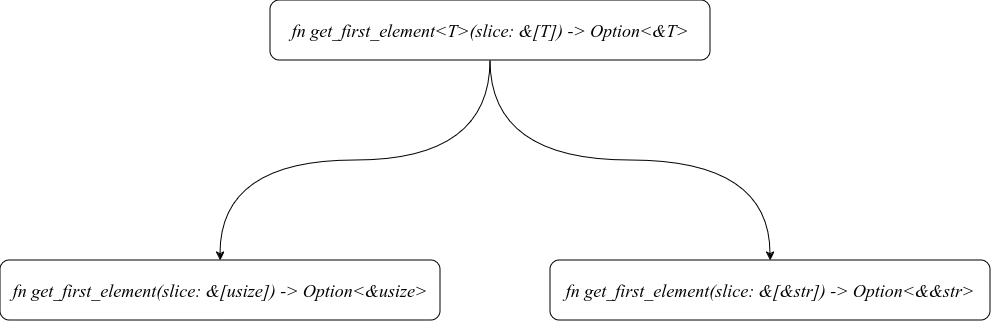
\includegraphics[scale=0.3]{images/rust/rust_generics}
  \caption{Παράδειγμα μεταγλώττισης generics.}
  \label{fig:rust_generic}
\end{figure}

Μπορούμε να περιορίσουμε το σύνολο των πιθανών τιμών ανάλογα με τα
traits (ουσιαστικά interfaces της Java) που υλοποιεί το generic. Για
παράδειγμα, αν θέλουμε μια συνάρτηση να μπορεί να χρησιμοποιεί μόνο
τύπους δεδομένων που υλοποιούν το trait \verb|Display|:

\begin{lstlisting}[language=Rust]
use std::fmt::Display;

fn print_element<T: std::fmt::Display>(element: T) {
    println!("Element: {}", element);
}

fn main() {
    print_element(42);        // i32 implements Display
    print_element("hello");   // &str implements Display
    print_element(vec![1, 2, 3]); // Error: Vec does not implement Display
}
\end{lstlisting}

Το μοντέλο async στην Rust βασίζεται στα Futures τα οποία με την σειρά
τους στηρίζονται πολύ στα generics. Τα Futures είναι traits 
και αντιπροσωπεύουν τιμές που δεν είναι άμεσα διαθέσιμες αλλά θα γίνουν ενδεχωμένος κάποια στιγμή
στο μέλλον. Ο μεταγλωτιστής υλοποιεί τα Futures ως state machines τα οποία δεν τρέχουν κατά
την διάρκεια της εκτέλεσης αλλά καταλήγουν ενσωματωμένα στο τελικό binary ως loops και jumps.

Ένα απλό παράδειγμα χρήσης async είναι το κλασσικό HTTP fetch:

\begin{lstlisting}[language=Rust]
async fn fetch_data(url: &str) -> Result<String, reqwest::Error> {
    let response = reqwest::get(url).await?;
    let body = response.text().await?;
    Ok(body)
}

#[tokio::main]
async fn main() {
    match fetch_data("http://example.com").await {
        Ok(body) => println!("Response: {}", body),
        Err(e) => println!("Error: {:?}", e),
    }
}
\end{lstlisting}

Το γεγονός ότι τα \verb|async| σύμβολα είναι compile time οντότητες αφαιρεί
ένα τεράστιο overhead που έρχεται με την υλοποίηση των παραδοσιακών runtimes.

Για να κατανοήσουμε πλήρως αυτόν μηχανισμό πρέπει να εξετάσουμε πώς αποσαφηνίζεται
(desugar) ένα async block. Στο ενδιάμεσο στάδιο HIR οτιδήποτε σύμβολο είναι \verb|async|
μεταφράζεται στην πρωτόγονη μορφή του, δηλαδή ένα Future με μια generic παράμετρο.

Το Future trait φαίνεται κάπως έτσι:

\begin{lstlisting}[language=Rust]
pub trait Future<Output> {
    // Required method
    fn poll(self: Pin<&mut Self>, cx: &mut Context<'_>) -> Poll<Output>;
}
\end{lstlisting}

Κατά συνέπεια η ταυτότητα της συνάρτησης fetch αποσαφηνίζεται από

\begin{lstlisting}[language=Rust] 
async fn fetch_data(url: &str) -> Result<String, reqwest::Error>
\end{lstlisting}

σε

\begin{lstlisting}[language=Rust] 
fn fetch_data<F: Future<Result<String,reqwest::Error>>>(url: &str) -> F
\end{lstlisting}

Παράλληλα το ενσωματωμένο μέρος της συνάρτησης αντικαθιστά τα \verb|await|
με την μέθοδο \verb|poll| 

\begin{lstlisting}[language=Rust] 
fn fetch_data<F: Future<Result<String,reqwest::Error>>>(url: &str) -> F
    let response = reqwest::get(url).poll(someContext);
    let body = response.text().poll(someContext);
    Ok(body)
}
\end{lstlisting}

Προφανώς η υλοποίηση του Future trait και κατά συνέπεια της μεθόδου \verb|poll|
αλλάζει σε κάθε async οικοσύστημα. Η γενική ιδέα όμως είναι ότι η \verb|poll|
επιστρέφει την κατάσταση της συνάρτησης που καλείτε, δηλαδή:

\begin{enumerate}
  \item Αν περιμένει την σειρά της για το επόμενο κάλεσμα (Waiting).
  \item Αν βρίσκεται στην διαδικασία του καλέσματος (Pending).
  \item Αν είναι έτοιμη και έχει τελειώσει το κάλεσμα (Done). 
\end{enumerate}

Τα enums της Rust μοντελοποιούν τις καταστάσεις σχεδόν πάντα,
το παρακάτω παράδειγμα δεν θα κάνει compile για πολλούς λόγους
και μπορεί να θεωρηθεί ψευδοκώδικας.

\begin{lstlisting}[language=Rust]
  enum FetchDataState
  {
    Waiting,
    Pending,
    Done(Result<&str,reqwest::Error>),
  }
 
  enum RespDataState
  {
    Waiting,
    Pending,
    Done(Result<&str,reqwest::Error>),
  }

  struct get
  {
    state: FetchDataState,
    ...,
  }

  struct resp
  {
    state: RespDataState,
    ...,
  }
  
  impl<Output=Result<&str,reqwest::Error>> Future<Output> for get
  {
    fn poll(self: Pin<&mut Self>,cx: &mut Context<'_>) -> Poll<Output>
    {
      loop
      {
        match &mut this.state
        {
          FetchDataState::Waiting => Poll::Pending,
          FetchDataState::Pending => Poll::Pending,
          FetchDataState::Done(res) => Poll::Ready(res),
        }
      }
    }
  }
 
  impl<Output=Result<&str,reqwest::Error>> Future<Output> for resp
  {
    fn poll(self: Pin<&mut Self>,cx: &mut Context<'_>) -> Poll<Output>
    {
      loop
      {
        match &mut this.state
        {
          RespDataState::Waiting => Poll::Pending,
          RespDataState::Pending => Poll::Pending,
          RespDataState::Done(res) => Poll::Ready(res),
        }
      }
    }
  }
\end{lstlisting}

Μια καλή ερώτηση σε αυτό το σημείο είναι πιο το νόημα? Στο παραπάνω παράδειγμα
είναι ξεκάθαρο ότι δεν γίνεται τίποτα παράλληλα απλώς ελέγχουμε αν η συνάρτηση
έχει τελειώσει και πράγματι αυτή είναι η περίπτωση.

Τα Futures δεν είναι τίποτα χωρίς έναν εκτελεστή (Executor) ο οποίος μπορεί να αλλάζει
την συνάρτηση που καλείτε ανάλογα με το Context της. Ένας εκτελεστής αποτελείτε από
έναν Spawner που προσθέτει ή αφαιρεί συναρτήσεις που επιστρέφουν Futures και έναν Waker
που "ξυπνάει" τις συναρτήσεις από τον Spawner για να ελέγξει την κατάσταση τους.

Στην παρακάτω υλοποίηση ψευδοκώδικα ο εκτελεστής είναι απλώς μια δυναμική λίστα και ο
Spawner μια συνάρτηση που προσθέτει Tasks. 

\begin{lstlisting}[language=Rust]
struct Executor {
    queue: VecDeque<Task>,
}

impl Executor {
    fn new() -> Self {
        Executor {
            queue: VecDeque::new(),
        }
    }

    fn spawn(&mut self, task: Task) {
        self.queue.push_back(task);
    }

    fn run(&mut self) {
        while let Some(mut task) = self.queue.pop_front() {
            let waker = task.get_waker();
            let mut context = Context::from_waker(&waker);
            match task.future.as_mut().poll(&mut context) {
                Poll::Pending => self.queue.push_back(task),
                Poll::Ready(_) => {},
            }
        }
    }
}

struct Task {
    future: Pin<Box<dyn Future<Output = ()>>>,
}

impl Task {
    fn get_waker(&self) -> Waker {
      //Wake the task
    }
}

fn main() {
    let mut executor = Executor { queue: VecDeque::new() };

    executor.queue.push_back(Task::new(fetch_data("http://example.com")));

    executor.run();
}
\end{lstlisting}

Για λόγους αισθητικής τις περισσότερες φορές χρησιμοποιούνται macros τα οποία
κρύβουν την πραγματική λειτουργία του executor. Τα macros στην Rust είναι πάρα
πολύ έξυπνα και μπορούν να διαβάσουν πρακτικά όλο το συντακτικό της γλώσσας. Κατά
συνέπεια μια συνάρτηση για παράδειγμα με τον εκτελεστή της embassy φαίνεται έτσι:

\begin{lstlisting}[language=Rust]
#[esp_hal_embassy::main]
async fn main(spawner: Spawner)
{
  //do stuff
  //spawn tasks
  spawner.spawn(task1()).ok();
  spawner.spawn(task2()).ok();
}
\end{lstlisting}

Προφανώς εδώ δεν φαίνεται να ορίζουμε κανέναν εκτελεστή και δεν
υπάρχει καμία λούπα που να τρέχει τα tasks. Για τις περισσότερες
εφαρμογές αυτό είναι ίσως πιο επιθυμητό στην δικιά μας περίπτωση όμως
θέλουμε τα τρέχουμε χρονομετρητές πριν και μετά από κάθε poll που εκτελείται. Ήμαστε
αναγκασμένοι λοιπόν να αποσαφηνίσουμε τα macros όσο το δυνατόν γίνεται:

\begin{lstlisting}[language=Rust]
#[main]
fn main() -> ! {
    let executor = EXECUTOR.init(Executor::new(3 as *mut ()));
    let spawner = executor.spawner();
    spawner.spawn(task1()).ok();
    spawner.spawn(task2()).ok();
    // let mut sleep_tick_count = 0;
    let mut acc = 0.0;
    let start_time = Instant::now();
    loop {
        let start_pol_time = Instant::now();
        unsafe { executor.poll() };
        let end_pol_time = Instant::now();
        let elapsed_pol = end_pol_time.duration_since(start_pol_time) as f64;
        acc += elapsed_pol_time;
        let total_elapsed = start_time.elapsed().as_ticks() as f64;
        let cpu_usage = acc * 100_f64 / total_elapsed
        //do stuff with cpu usage
    }
}
\end{lstlisting}

Στον παραπάνω κώδικα η loop είναι η αντίστοιχη συνάρτηση \verb|run| του ψευδοκώδικα
η μόνη διαφορά είναι ότι δεν κάνουμε χειροκίνητα την επιλογή των task που θα τρέξει
μέσο του Context. Στην πραγματικότητα το "Context" μπορεί να σημαίνει πολλά πράγματα,
είναι απλώς ένας δείκτης που αντιπροσωπεύει διαφορετικά δεδομένα ανάλογα με την τιμή του.
Εδώ επιλέχθηκε η τιμή $3$ διαβάζωντας το source-code του εκτελεστή και συμπεραίνοντας
ότι αυτή είναι η εντολή που αρχικοποιεί τον executor. Όταν καλούμε την \verb|poll|
προφανώς καλούνται εσωτερικά όλες οι συναρτήσεις που έχουν γίνει spawn. 

\subsubsection{HAL Patterns}

Προφανώς κάθε MCU είναι διαφορετικό και διαθέτει διαφορετικά περιφερειακά,
ποίκιλες δυνατότητες,
λιγότερα ή περισσότερα GPIO Pins etc. Το embedded-hal είναι μια συλλογή
traits που αποσκοπούν στην μοντελοποίηση ενός abstract MCU. Υπάρχουν traits
για προτόκκολα επικοινωνίας όπως UART και I2C αλλά και traits για λειτουργεία
των GPIO, PWM και οτιδήποτε άλλο είναι πιθανό να χρειαστούμε.
Όπως έχουμε δει όμως τα traits δεν είναι τίποτα παραπάνω από πρότυπα, χρειαζόμαστε
λοιπόν μια υλοποίηση των traits για τον δικό μας μικροελεγκτή. Θα μπορούσαμε για την
συγκεκριμένη εργασία να κάνουμε τις δικές μας υλοποιήσεις, και θα γίνει αυτό σε έναν
βαθμό αλλά υπάρχει ήδη το crate esp-hal το οποίο όχι μόνο προσφέρει υλοποιήσεις για αυτά τα traits
αλλά παρέχει ένα struct, το Peripherals το οποίο μοντελοποιεί τα περιφερειακά του ESP.

\begin{figure}[htb!]
  \centering
  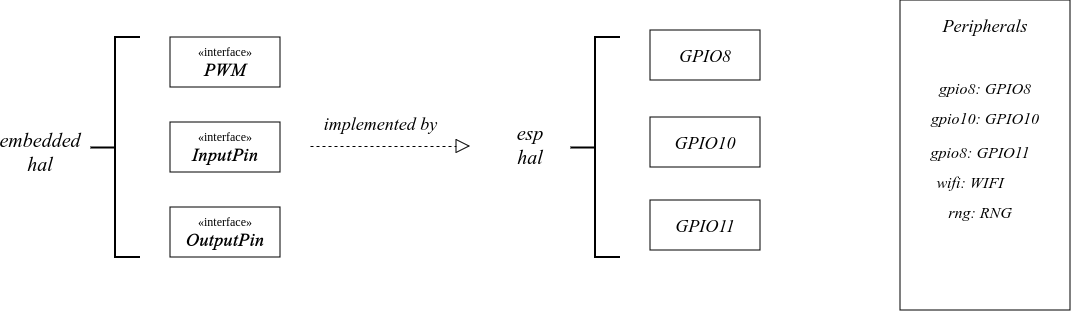
\includegraphics[scale=0.4]{images/rust/peripheral_pattern.drawio.png}
  \caption{HAL Pattern για τον ESP.}
  \label{fig:peripheral_pattern}
\end{figure}

Το \verb|Peripherals| struct υλοποιείται διαφορετικά ανάλογα με τον
μικροελεγκτή. Δηλαδή κάνουμε compile το esp-hal με ένα flag που
αντιπροσωπεύει το όνομα του MCU που χρησιμοποιούμε. Στo cargo, το αντίστοιχο
CMake της Rust, τα flags λέγονται features και γράφονται σε ένα αρχείο Cargo.toml
που βρίσκεται στο root του project:

\begin{lstlisting}
  [dependencies]
  ...other deps
  esp-hal = { version = "0.23.1", features = ["esp32c6", "unstable"] }
\end{lstlisting}

Η προσέγγιση του Peripheral ακολουθεί τις αρχές της
Rust που αναλύσαμε παραπάνω δηλαδή στο ότι κάθε περιφεριακό (USB
Port,GPIO-Pins,SPI,UART) αποτελεί έναν μοναδικό και καταναλώσιμο πόρο.
Κατά συνέπεια, μόλις το περιφερειακό ληφθεί από τη δομή που το
διαχειρίζεται (συνήθως μια δομή τύπου Peripherals), θεωρείται ότι
καταναλώθηκε και δεν μπορεί να χρησιμοποιηθεί ξανά χωρίς ρητή
επιστροφή του ελέγχου από το πρόγραμμα. Για παράδειγμα, ένα GPIO pin
(ψηφιακή θύρα εισόδου/εξόδου) μπορεί να χρησιμοποιηθεί είτε για είσοδο
είτε για έξοδο, αλλά ποτέ ταυτόχρονα, καθώς η πρώτη χρήση καταναλώνει
τον αντίστοιχο πόρο.




\newpage    
\subsection{Γράφοντας το Project}

Θα δούμε πως η υλοποίηση του Project με βάση το specification που
έχουμε θέσει είναι ιδιαίτερα απλή. Παρόλα αυτά δεν προσφέρονται βιβλιοθήκες
για τον HC-SR04 όπως στην περίπτωση του ESP-IDF. Παράλληλα το API της
βιβλιοθήκης του MQTT είναι πολύ δύσκολα διαχειρήσημο οπότε θα
χρειαστεί κάποιου είδους βελτίωση χωρίς απαραίτητα να γράψουμε το
πρωτόκολλο από την αρχή (το οποίο όμως φαίνεται να είναι η ιδανική
λύση). Με βάση την γνώση που έχουμε δώσει στην εισαγωγή αυτού του
κεφαλαίου όμως γίνεται ξεκάθαρο πως αυτό δεν αποτελεί πρόβλημα καθώς η
εκφραστηκότητα της Rust κάνει το γράψιμο κώδικα να φαίνεται σαν πολύ
οργανική διαδικασία.

Μια επιλογή για να ξεκινήσουμε είναι να δημιουργήσουμε ένα Cargo.toml και
να θέσουμε τις βιβλιοθήκες που θέλουμε να μεταγλωττίσουμε μαζί με το Project.
Όμως υπάρχει μια καλύτερη λύση, το \verb|esp-generate --chip esp32c6 my_project|
δημιουργεί τα απαραίτητα αρχεία με τις βιβλιοθήκες που είναι απαραίτητες ανάλογα με
τις ρυθμίσεις μας. Προφανώς αν θέλουμε προσθέτουμε κιάλλες μπορούμε είτε από ένα τερματικό
\verb|cargo add library| είτε με το συντακτικό TOML που έχουμε δείξει παραπάνω.
Το τελικό directory έχει της εξής δομή:

\begin{figure}[htbp]
  \centering
\begin{forest}
for tree={
  font=\ttfamily,
  grow'=0,
  child anchor=west,
  parent anchor=south,
  anchor=west,
  calign=first,
  edge path={
    \noexpand\path [draw, \forestoption{edge}]
      (!u.south west) +(5pt,0) |- (.child anchor)\forestoption{edge label};
  },
  before typesetting nodes={
    if n=1
      {insert before={[,phantom]}}
      {}
  },
  fit=band,
  before computing xy={l=15pt},
}
[.
  [build.rs]
  [.cargo
    [config.toml]
  ]
  [Cargo.toml]
  [.gitignore]
  [rust-toolchain.toml]
  [src
    [bin
      [main.rs]
    ]
    [lib.rs]
  ]
]
\end{forest}
\caption{Project folder structure.}
\label{fig:project_structure}
\end{figure}

Το project θα αποτελείτε από δύο δικές μας βιβλιοθήκες που θα είναι υπεύθυνες για:

\begin{enumerate}
  \item Την λειτουργία του αισθητήρα απόστασης.
  \item Την λειτουργεία του πρωτόκολλου MQTT.
\end{enumerate}

\subsubsection{HC-SR04 Driver}

Ο σένσορας για να λειτουργήσει χρειάζεται εκτός από το VCC και το ground pin
ένα input και ένα output. Οπότε γράφουμε σε ένα αρχείο \verb|hcsr04.rs|:

\begin{lstlisting}[language=Rust]
pub struct HCSR04<'h, Clock: Timer> {
    trigger: Output<'h>,
    echo: Input<'h>,
    clock: Clock,
}
\end{lstlisting}

Ήδη αρκετά κομμάτια στον κώδικα έχουν ιδιαίτερο ενδιαφέρον.

Αρχικά παρατηρούμε ότι δεν χρησιμοποιούμε συγκεκριμένο τύπο για
GPIO pins. Χρησιμοποιώντας \verb|Input| και \verb|Output| όχι μόνο
μοντελοποιούμε καλύτερα τον αισθητήρα αλλά αποφεύγουμε μελλοντικά
runtime errors αν αφήναμε τον χρήστη να προσθέσει ότι pins ήθελε με
τις δικές του ρυθμίσεις. Με αυτόν τον τρόπο εκφράζουμε "ο αισθητήρας καταναλώνει
ένα output και ένα input pin".

Με την ίδια λογική ορίζουμε μια generic παράμετρο Clock η οποία περιορίζεται
στους τύπους που υλοποιούν το \verb|Timer| trait. Αφήνουμε λοιπόν στον
χρήστη να επιλέξει το ρολόι που θα χρησιμοποιήσει εφόσον οι περισσότεροι
μικροελεγκτές έχουν πολλά και ανάλογα με τους σκοπούς τα αποτελέσματα
μπορούν να διαφέρουν. Για τον ESP, αν μας ενδιαφέρει πάρα πολύ η εγκυρότητα των τιμών
του χρονομετρητή τότε συνήθως θέλουμε το system timer αλλιώς μπορούμε να επιλέξουμε
ένα από τα Timer Groups που προσφέρει ο ESP ή ένα software timer της embassy το οποίο
προφανώς βασίζεται σε ένα από τα παραπάνω.

Το συντακτικό \verb|<'h>| έχει να κάνει με τον χρόνο ζωής (lifetime)
των πεδίων στο εσωτερικό του struct. Η πλήρης ανάλυση των lifetimes
είναι εκτός των πλαισίων της εργασίας αλλά ουσιαστικά αυτό που
εκφράζουν είναι για πόσο χρόνο κατά την εκτέλεση του προγράμματος ζει
ένα σύμβολο. Στην συγκεκριμένη περίπτωση όλα ζουν για το ίδιο χρόνικό
διάστημα, μέχρι ο HCSR04 να βγει από το scope.

Όσο αναφορά τις μεθόδους του struct τις γράφουμε μέσα σε ένα \verb|impl|
block που διαθέτει τις κατάλληλες μεταβλητές. Τα \verb|impl| blocks εκφράζουν
το πιο μέθοδοι ορίζονται για έναν τύπο $T$.

\begin{lstlisting}[language=Rust]
  impl<'h,Clock: Timer> HCSR04<'h, Clock>
  {
    //Methods go here
  }
\end{lstlisting}

Οι μεταβλητές αυτές είναι όσο πιο γενικές δυνατόν γίνεται. Θα μπορούσαμε
κάλιστα να ορίσουμε ένα πιο περιορισμένο implementation. Για παράδειγμα να
ορίσουμε μεθόδους μόνο για τα HCSR04 που έχουν για χρονομετρητή ένα \verb|Alarm|:

\begin{lstlisting}[language=Rust]
  impl<'h> HCSR04<'h, Alarm>
  {
    //Methods go here
  }
\end{lstlisting}

Χρειαζόμαστε προφανώς μια συνάρτηση για να δημιουργήσουμε
το αντικείμενο που αντιπροσωπεύει τον αισθητήρα.

\begin{lstlisting}[language=Rust]
//inside the impl block
pub fn new<TRIG: PeripheralOutput + OutputPin, ECHO: PeripheralInput + InputPin>(
trigger: impl Peripheral<P = TRIG> + 'h,
echo: impl Peripheral<P = ECHO> + 'h,
timer: Clock,
) -> Self {
Self {
    trigger: Output::new(trigger, Level::Low),
    echo: Input::new(echo, Pull::None),
    clock: timer,
}
}
\end{lstlisting}

Η συνάρτηση έχει δύο παραμέτρους που είναι generic και πρέπει
να κάνουν implement το Peripheral trait (διαφορετικό από το Peripheral struct).

\begin{enumerate}
\item Η trigger είναι μια παράμετρος που κάνει implement το Peripheral
  και είναι PeripheralOutput + OutputPin. Δηλαδή αναγκάζουμε την συνάρτηση
  να δεχτεί GPIO Pins που λειτουργούν σαν outputs. Έστω ότι για κάποιο
  λόγο προσπαθήσουμε να καλέσουμε την συνάρτηση με trigger = VCC Pin
  το πρόγραμμα δεν θα κάνει compile επειδή το VCC Pin δεν κάνει implement
  το OutputPin.
\item Η echo είναι μια παράμετρος που κάνει implement το Peripheral
  και είναι PeripheralInput + InputPin. Δηλαδή αναγκάζουμε την συνάρτηση
  να δεχτεί GPIO Pins που λειτουργούν σαν inputs. Έστω ότι για κάποιο
  λόγο προσπαθήσουμε να καλέσουμε την συνάρτηση με echo = VCC Pin
  το πρόγραμμα δεν θα κάνει compile επειδή το VCC Pin δεν κάνει implement
  το InputPin.
\end{enumerate}

Η πιο ενδιαφέρουσα μέθοδος είναι αυτή που υπολογίζει την απόσταση:

\begin{lstlisting}[language=Rust]
//inside the impl block
pub fn measure_distance(&mut self) -> f64 {
    let delay = Delay::new();

    self.clock.start();
    //Send ultrasonic wave
    self.trigger.set_high();
    delay.delay_micros(10);
    self.trigger.set_low();
    //Ultra sonic wave is sent

    //Wait until echo bounces back
    while self.echo.is_low() {
        //DO NOT DEOPTIMIZE THE LOOP AWAY
        unsafe { asm!("nop") };
    }

    //Start timing start = CURRENT_TIME
    let start = self.clock.now();

    //Wait until echo pin returns to low
    while self.echo.is_high() {
        //DO NOT DEOPTIMIZE THE LOOP AWAY
        unsafe { asm!("nop") };
    }

    //End timing end = CURRENT_TIME > start
    let end = self.clock.now();

    let pulse_duration = (end - start).to_micros();

    //return the distance
    pulse_duration as f64 / 58_f64
}
\end{lstlisting}

\subsubsection{MQTT Driver}
Goodbye
\subsubsection{Main Program}
Hellogoodbye




\newpage

\appendix

\newpage

\printbibliography

\end{document}
